% !TEX TS-program = pdflatex
% !TEX encoding = UTF-8 Unicode

% This file is a template using the "beamer" package to create slides for a talk or presentation
% - Talk at a conference/colloquium.
% - Talk length is about 20min.
% - Style is ornate.

% MODIFIED by Jonathan Kew, 2008-07-06
% The header comments and encoding in this file were modified for inclusion with TeXworks.
% The content is otherwise unchanged from the original distributed with the beamer package.

\documentclass{beamer}
\usepackage{hyperref}

%This file is released under (CC BY-SA 4.0) license. See the following website for details http://creativecommons.org/licenses/by-sa/4.0/legalcode


\mode<presentation>
{
  \usetheme{Warsaw}
  % or ...

  %\setbeamercovered{transparent}
  % or whatever (possibly just delete it)
}



\usepackage[english]{babel}
% or whatever

\usepackage[utf8]{inputenc}
% or whatever
\usepackage[graphics]{}
\usepackage[amsmath]{}
\usepackage{times}
\usepackage[T1]{fontenc}
% Or whatever. Note that the encoding and the font should match. If T1
% does not look nice, try deleting the line with the fontenc.


\title[PSD with Arduino CC-BY-SA.4.0] % (optional, use only with long paper titles)
{The trials and tribulations of building a phase-sensitive detector with an Arduino microcontroller}


\author[K.\ D.\ Schultz] % (optional, use only with lots of authors)
{K.~D.~Schultz}
% - Give the names in the same order as the appear in the paper.
% - Use the \inst{?} command only if the authors have different
%   affiliation.

\institute[Hartwick College] % (optional, but mostly needed)
{
 
  Department of Physics\\
  Hartwick College
}
% - Use the \inst command only if there are several affiliations.
% - Keep it simple, no one is interested in your street address.

\date[MAS-APS] % (optional, should be abbreviation of conference name)
{MAS-APS, 2014}
% - Either use conference name or its abbreviation.
% - Not really informative to the audience, more for people (including
%   yourself) who are reading the slides online

% This is only inserted into the PDF information catalog. Can be left
% out. 



% If you have a file called "university-logo-filename.xxx", where xxx
% is a graphic format that can be processed by latex or pdflatex,
% resp., then you can add a logo as follows:

 \pgfdeclareimage[height=0.5cm]{university-logo}{HartwickLogo}
 \logo{\pgfuseimage{university-logo}}



% Delete this, if you do not want the table of contents to pop up at
% the beginning of each subsection:
%\AtBeginSubsection[]
%{
%  \begin{frame}<beamer>{Outline}
%    \tableofcontents[currentsection,currentsubsection]
%  \end{frame}
%}


% If you wish to uncover everything in a step-wise fashion, uncomment
% the following command: 

%\beamerdefaultoverlayspecification{<+->}


\begin{document}

\begin{frame}
  \titlepage
\end{frame}

%\begin{frame}{Outline}
%  \tableofcontents
%  % You might wish to add the option [pausesections]
%\end{frame}


% Structuring a talk is a difficult task and the following structure
% may not be suitable. Here are some rules that apply for this
% solution: 

% - Exactly two or three sections (other than the summary).
% - At *most* three subsections per section.
% - Talk about 30s to 2min per frame. So there should be between about
%   15 and 30 frames, all told.

% - A conference audience is likely to know very little of what you
%   are going to talk about. So *simplify*!
% - In a 20min talk, getting the main ideas across is hard
%   enough. Leave out details, even if it means being less precise than
%   you think necessary.
% - If you omit details that are vital to the proof/implementation,
%   just say so once. Everybody will be happy with that.

\section {Introduction}

\subsection{Original Goals}

\begin{frame}
\frametitle{Original Goals}

\begin{itemize}%[<+-|alert@+>]
\item {Use Arduino as a tool for teaching about phase-sensitive detection.}
\item{To do so with only the Arduino, a computer for display purposes, and passive external components (resistors and capacitors)}

\end{itemize}
\end{frame}

\subsection{Motivation}
\begin{frame}
\frametitle{Why PSD?}
\begin{itemize}%[<+-| alert@+>]
\item{Phase Sensitive Detection (PSD) is the basis of many techniques in physics and engineering}
\begin{itemize}
\item{Homodyne detection}
\item{Interferometry}
\item{Lock-in amplifiers}

\end{itemize}

\item {Black boxes are useful for application work, but not so much for pedagogical purposes}
\item {Software PSD allows students to peek into the black box.}


\end{itemize}

\end{frame}
\begin{frame}
\frametitle{Why Arduino?}
\begin{columns}[t]
\column[c]{0.6\textwidth}
\begin{itemize}
\item{Cheap}
\item {Popular}
\begin{itemize}
\item {Lots of support}
\end{itemize}
\item {Simple programming environment}
\begin{itemize}
\item {Perhaps too simple, IDE has very poor debugging tools.}
\end{itemize}
\item{Works well with Processing, which is a free and powerful language for visualization}
\item{Both Arduino and Processing are platform agnostic: Windows, Linux, OS X, Raspberry Pi...}
\end{itemize}
\column[c]{0.4\textwidth}
\begin{figure}
\hspace*{-.75cm}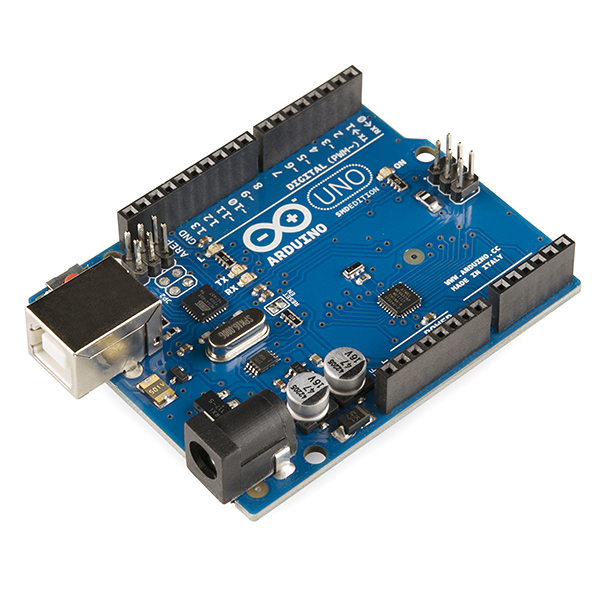
\includegraphics[scale=.25]{Arduino_Uno_-_R3.jpg}\\
\tiny {Arduino picture from Sparkfun CC-BY-2.0}
\end{figure}
\end{columns}
\end{frame}



\subsection{Background Material}
\begin{frame}
\frametitle{PSD Basics}


\begin{columns}[t]
	\column[c]{4.5cm}
	    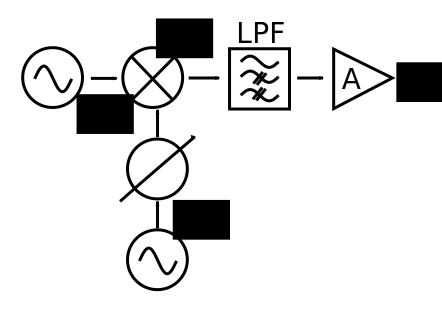
\includegraphics[height=3.2cm]{PSD_block}
	\column[c]{6.6cm}
\small	
	\begin{block}{Mathematics of PSD}
	
	\begin{align*}
	V_{mix}&=V_s V_r \left [ ( \cos\left(\omega_s-\omega_r\right)t-(\phi_s-\phi_r)\right]\\
	V_o&=A \frac{V_s V_r}{2} \left[ \cos(\phi_s-\phi_r)\right]
	\end{align*}
	
	\end{block}

\begin{block}{Restrictions}
\begin{itemize}
\item $\omega_r=\omega_s$
\item\alert{ $V_s$ and $V_r$ have no DC offset}
\end{itemize}
\end{block}

\end{columns}
\end{frame}

\section{Is This Even Possible?}

%\begin{frame}
%\frametitle{What do we need? Can we do it?}
%\begin{columns}
%\column[T]{.5\textwidth}
%\begin{block}{Needed features}
%\begin{enumerate}
%
%\item {Generate reference signal.}
%\item {Adjustable phase to maximize signal.}
%\item {Get signal into Arduino}
%\item {Mix signal and reference and filter the results}
%\item {Display results}
%\end{enumerate}
%\end{block}
%\pause
%\column[T]{.5\textwidth}
%\begin{block}{Issues}
%\begin{enumerate}%[<+->]
%\item{Arduino has no analog out}
%\item{Shifting phase is difficult to do internally}
%\item{Positive voltages only}
%\item{Limited variable memory on Arduino}
%\item{Need to use serial over USB to Processing}
%\end{enumerate}
%\end{block}
%\end{columns}
%\end{frame}


\begin{frame}
\frametitle{Flowchart}
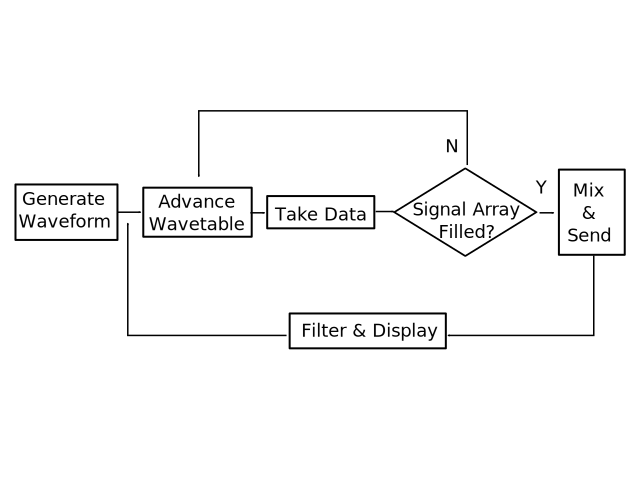
\includegraphics[scale=.5]{PSD_flowchart1}
\end{frame}

\subsection{Making it Work}
\begin{frame}
\frametitle{Phase Manipulation}
\begin{columns}[t]
\column[c]{0.3\textwidth}
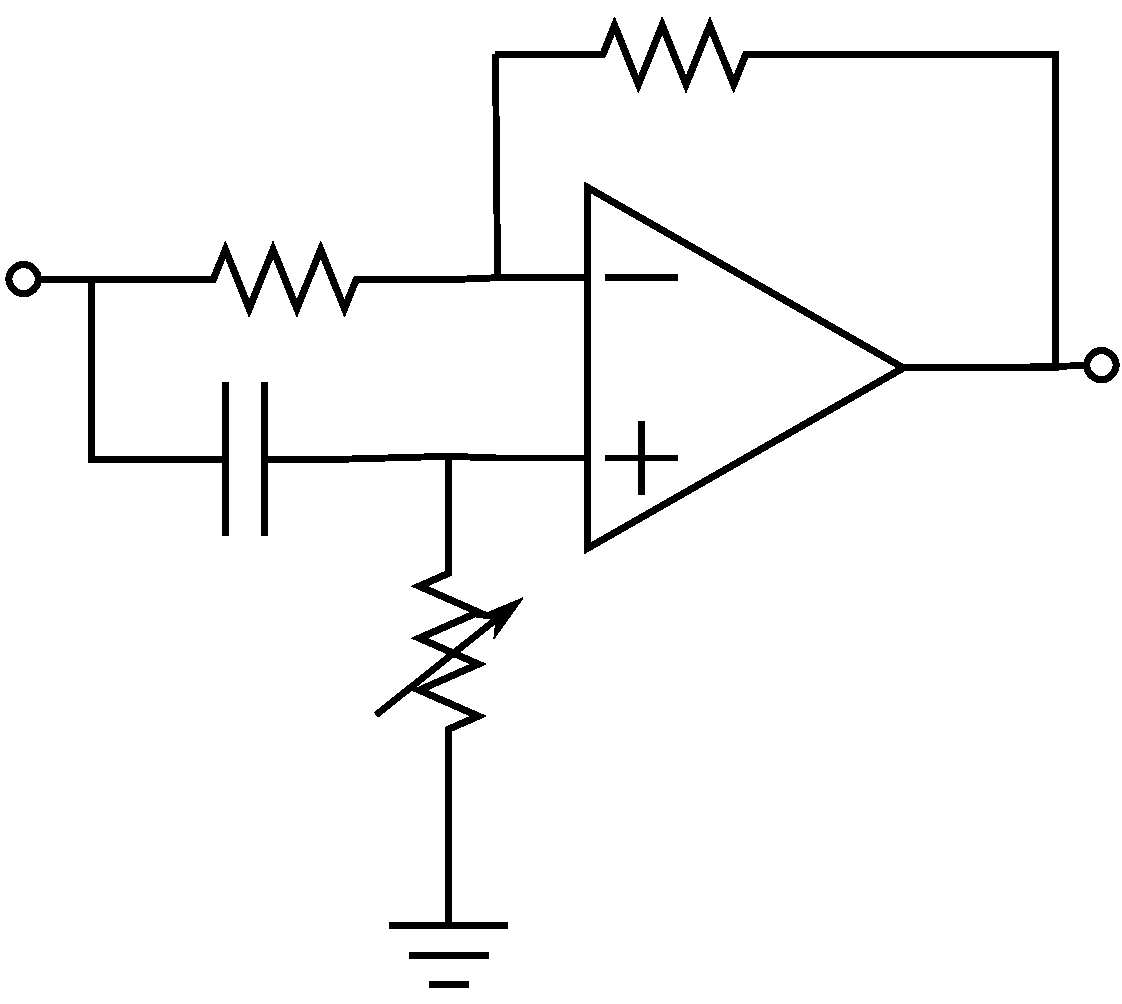
\includegraphics[scale=.2]{PhaseShift}

\column[c]{0.7\textwidth}

\begin{itemize}
\item {Need to be able to shift phase to maximize signal}
\item {All-pass phase shifters work, but require a bit more hardware external to Ardunio}
\item {Software solutions difficult to implement}
\item {Use two phase detection.}
	\begin{itemize}
	\item $V_I=V_s\times \cos(\theta), V_Q=V_s\times\sin(\theta)$
	\item $R=\sqrt{V_I^2+V_Q^2}$
	\item $\phi=\tan^{-1}(V_Q/V_I)$
	\end{itemize}
\end{itemize}

\end{columns}
\end{frame}

\begin{frame}
\frametitle{Creating a Reference Signal}
\begin{columns}[t]
	\column[c]{6cm}
	\begin{figure}
	    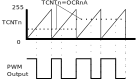
\includegraphics[scale=1.25]{Bitbang}\\
	    \tiny{ Picture adapted from J. Thompson, MAKE vol. 35}
	    \end{figure}
	    
	\column[c]{5cm}

	\begin{block}{Timers and Interrupts Part I}
	\begin{itemize}
	\item {The ratio of PWM on to off determines an average ``DC'' signal}
	\item{When register TCNT1 reaches OCR1A PWM goes low}
	\item {When TCNT1 overflows PWM goes high again}
	\end{itemize}
	
	\end{block}
\end{columns}
\end{frame}

\begin{frame}
\frametitle{Creating a Reference Signal}
\begin{columns}[T]
	\column[T]{.4\textwidth}
	\vspace{.5cm}
	   \begin{figure}
	    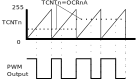
\includegraphics[scale=1.25]{Bitbang}\\
	    \tiny {Picture adapted from J. Thompson, MAKE vol. 35}
	    \end{figure}
	    \vspace{.3cm}
	    \begin{block}
	    $f_{ref}=\frac{\text{TCNT2 rate}}{\text{OCR2A value}\times\text{wavetable length}}$
	    \end{block}
	\column[T]{.5\textwidth}

	\begin{block}{Timers and Interrupts Part II}
	\begin{itemize}
	\item {Need fast timer2 and regular timer1, which outputs PWM}
	\item{When timer2 reaches OCR2A:}
	\begin{itemize}
        \item {Update OCR1A from wavetable}
        \item{ read signal at AnalogIn}
	\end{itemize}
	\item{When timer1 counts up to OCR1A, PWM goes low}
	\item {When timer1 overflows PWM goes high again}
	
	\end{itemize}
	
	\end{block}
\end{columns}
\end{frame}

\begin{frame}
\frametitle{Signal Input}
\begin{center}
\hspace*{-.45cm}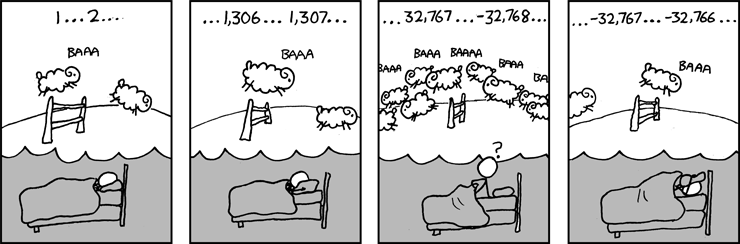
\includegraphics[scale=.5]{cant_sleep.png}
\end{center}
\end{frame}
\begin{frame}
\frametitle{Signal Input}
\begin{itemize}
	\item {Arduino can only have positive voltages at its inputs or outputs}
		\begin{itemize}
			\item {Integer overflow when mixing}
			\item {Necessary DC offsets makes phase indefinite}
		\end{itemize}
	\item {Need to run ADC as fast as we can so as to to interfere with reference generation.}

		\begin{itemize}
			\item{Setting pre-scalars and registers can get sampling rates of 50k samples/sec. Not bad for  a 30 board!}
			\item{ADC has 10 bit resolution with adjustable $V_{ref}$, so resolution on the order of a millivolt is possible}
		\end{itemize}
\end{itemize}

\end{frame}



\begin{frame}
\frametitle{Display}
\begin{columns}
\column{.5\textwidth}
\begin{figure}
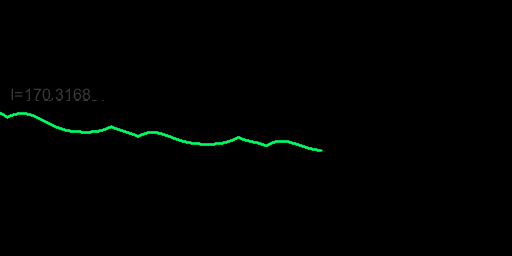
\includegraphics[scale=.3]{Snap.png}\\
In-phase channel as phase is changed
\end{figure}
\column{.5\textwidth}
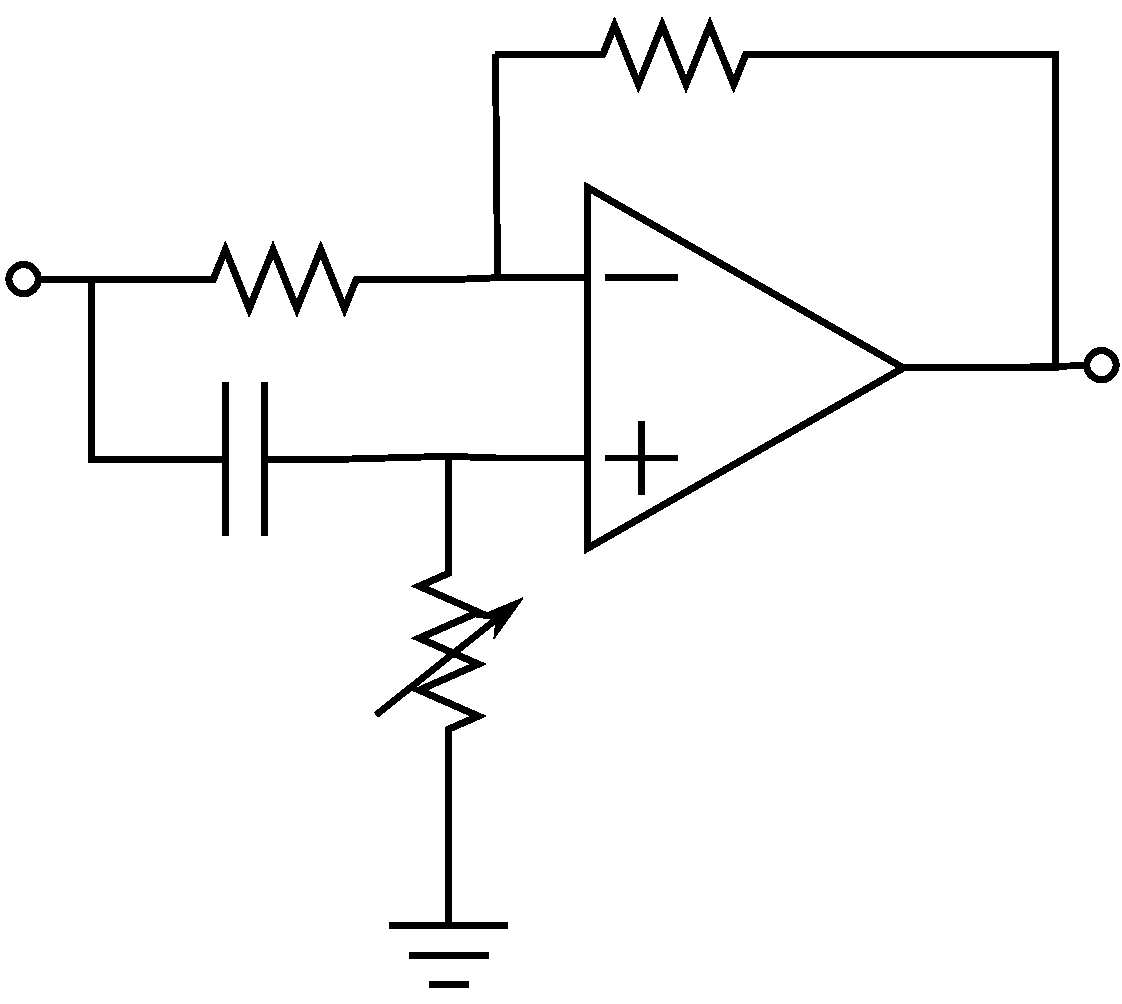
\includegraphics[scale=.3]{PhaseShift}
\end{columns}
\end{frame}



\section{Conclusions}
\begin{frame}
\begin{columns}
\column[T]{.5\textwidth}
\begin{block}{What we accomplished}
\begin{itemize}
\item {Built and tested a working two-channel phase-sensitive detector}
\item {Learned techniques that can be used for other micro-processor based instruments}
\item {Published on github under GPL v3 license}
\end{itemize}
\end{block}

\column[T]{.5\textwidth}
\begin{block}{Still to do}
\begin{itemize}
\item {Characterize detector (noise, internal phase shift, etc...)}
\item {Clean up display}
\item {Explore other memory options on Arduino}
\item {Use in an application}
\end{itemize}
\end{block}
\end{columns}
\end{frame}
% All of the following is optional and typically not needed. 
\appendix
\section<presentation>*{\appendixname}
\subsection<presentation>*{For Further Reading}

\begin{frame}[allowframebreaks]
  \frametitle<presentation>{For Further Reading}
    
  \begin{thebibliography}{10}
    
%  \beamertemplatebookbibitems
%  % Start with overview books.
%
%  \bibitem{Author1990}
%    A.~Author.
%    \newblock {\em Handbook of Everything}.
%    \newblock Some Press, 1990.
 
    
  \beamertemplateinternetbibitems
  % Followed by interesting articles. Keep the list short. 
\small{
  \bibitem{github2014}
    The programs!
    \newblock \url{https://github.com/HartwickChaosLab/Arduino-Phase-Sensitive-Detector}
   
   \bibitem{arduino}
   Arduino
   \newblock \url{http://www.arduino.cc}
   
   \bibitem{Processing}
   Processing
   \newblock \url{http://processing.org}
   
   \bibitem{measuring stuff}
   Moding the Arduino ADC
   \newblock \url{https://sites.google.com/site/measuringstuff/the-arduino}
  
   \beamertemplatearticlebibnitems
 
   \bibitem{Make35}
     J.~Thompson
     \newblock ``Advanced Arduino Sound Synthesis"
     \newblock Make Vol. 35 
   }
  \end{thebibliography}
\end{frame}

\end{document}


